\section{Designing a DC Power Supply System}

General purpose op-amps use bipolar power supply, typically $\pm$15 V. The common point between the +15V and -15V is the power supply common. This common is grounded and all voltage measurements are made with respect to this point.

Designing a power supply system which can give us such stable DC voltage outputs require multiple steps. Using a full-wave center tapped transformer, one can obtain +V, 0V and -V voltages. A typical power supply can have four major components:\\ 

\begin{enumerate}
    \item \textbf{Step-down transformer} to convert 220V AC to the required voltage.
    \item \textbf{Rectifier} to convert AC into DC.
    \item \textbf{Filtering} to remove ripples from the pulsating DC signal.
    \item \textbf{Voltage Regulator} (using a zener diode or otherwise) provides stability to the output voltage while load currents change.
\end{enumerate}

Additionally, some filtering can be done at the output to further smoothen the DC output, and act as a low pass filter.

\begin{figure}[H]
    \centering
    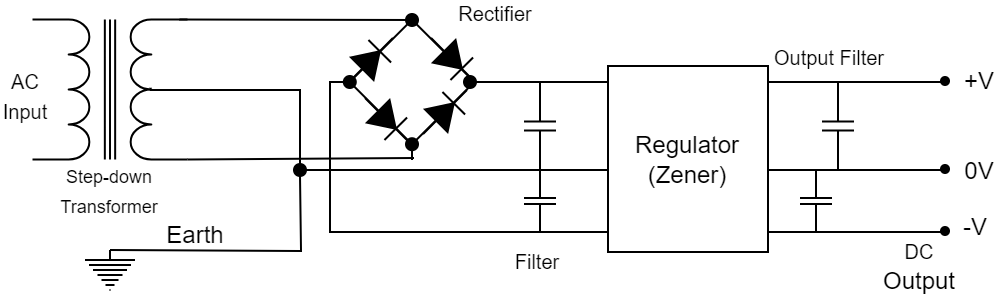
\includegraphics[width=1\columnwidth]{images/ps.drawio.png}
    \caption{Schematic diagram for a DC bipolar power supply system}
    \label{power supply}
\end{figure}

\section{Ground and Earthing}
Ground is a reference point in an electrical circuit from which voltages are measured. It can be thought of as a common return path for electrical current. There are several types of grounds,\\

\begin{enumerate}
    \item \textbf{Earth Ground:} Connecting the system to earth, i.e. a conductor buried in the ground usually using metal rods or wires, is called earthing. The ground pin on electrical outlets lead to this ground, and is intended to protect against insulation failure of the connected device.
    \begin{figure}[H]
        \centering
        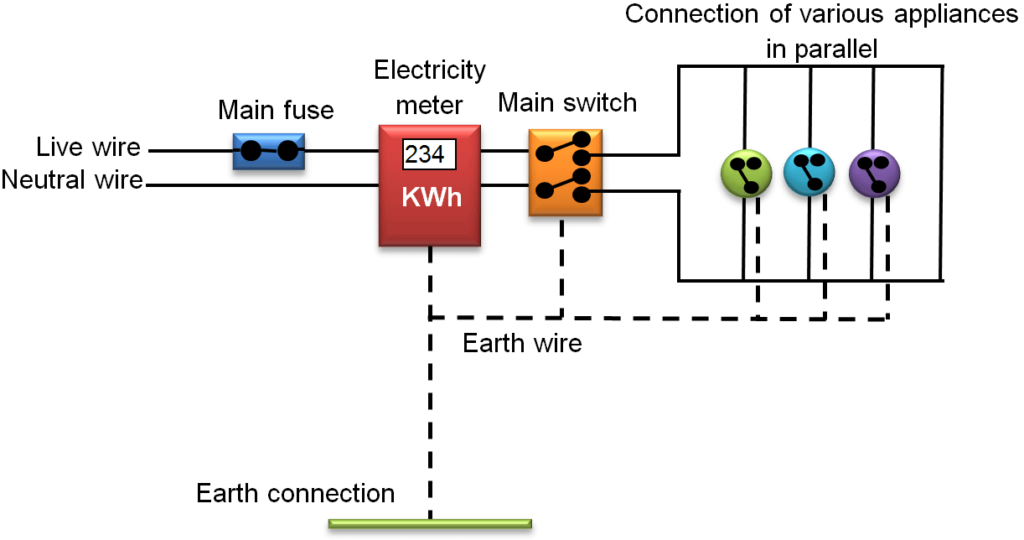
\includegraphics[width=0.85\columnwidth]{images/domestic.png}
        \caption{Schematic of a domestic power supply system showing the live neutral and earth connections.}
        \label{dom}
    \end{figure}
    There are essentially two types of earthing systems: (i) Copper earthing for active devices and (ii) Galvanised iron for body earthing. These are regularly kept in check to ensure $< 2$V potential difference between the neutral and earth wires in the electricity outlet. Some real-world earthing systems are shown in Fig. \ref{earth}.\\
    \item \textbf{Floating Ground:} It is essentially a ground that isn't actually attached to the earth, but to some other entity for electrical isolation.\\
    \item \textbf{Virtual Gound:} This is when a node of a circuit is maintained at a steady reference potential, without actually being connected directly to the reference potential. This is not an actual ground, but only a reference point. 
    
    In case of op-amps, when the non-inverting terminal is grounded then the inverting terminal will also act as ground, since they are at the same potential. Although the inverting terminal is not actually grounded, it acts as a virtual ground.\\
\end{enumerate}

\begin{figure}[H]
     \centering
     \begin{subfigure}[b]{0.2\textwidth}
         \centering
         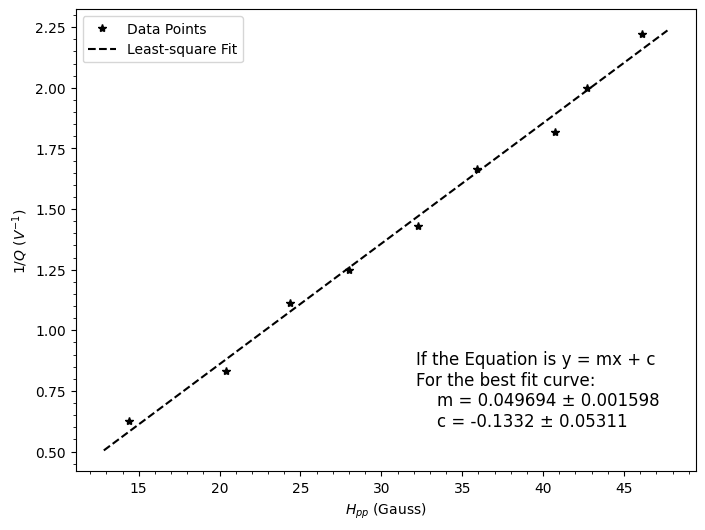
\includegraphics[width=\textwidth]{images/1.JPG}
     \end{subfigure}
     \hfill
     \begin{subfigure}[b]{0.25\textwidth}
         \centering
         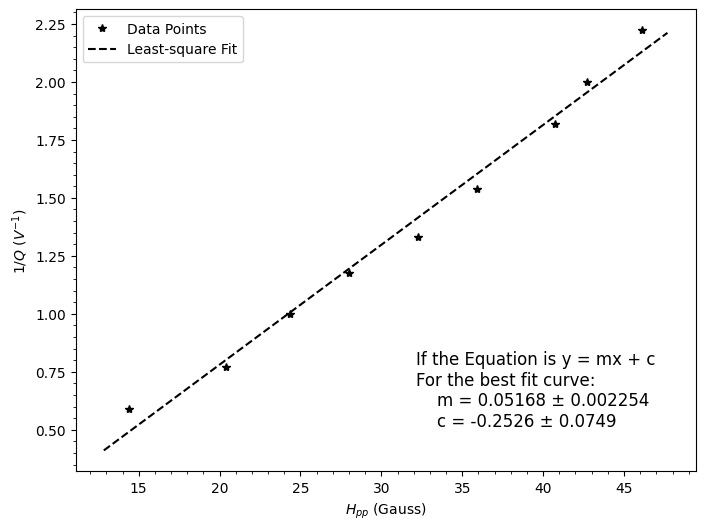
\includegraphics[width=\textwidth]{images/2.JPG}
     \end{subfigure}
     \begin{subfigure}[b]{0.25\textwidth}
        \centering
        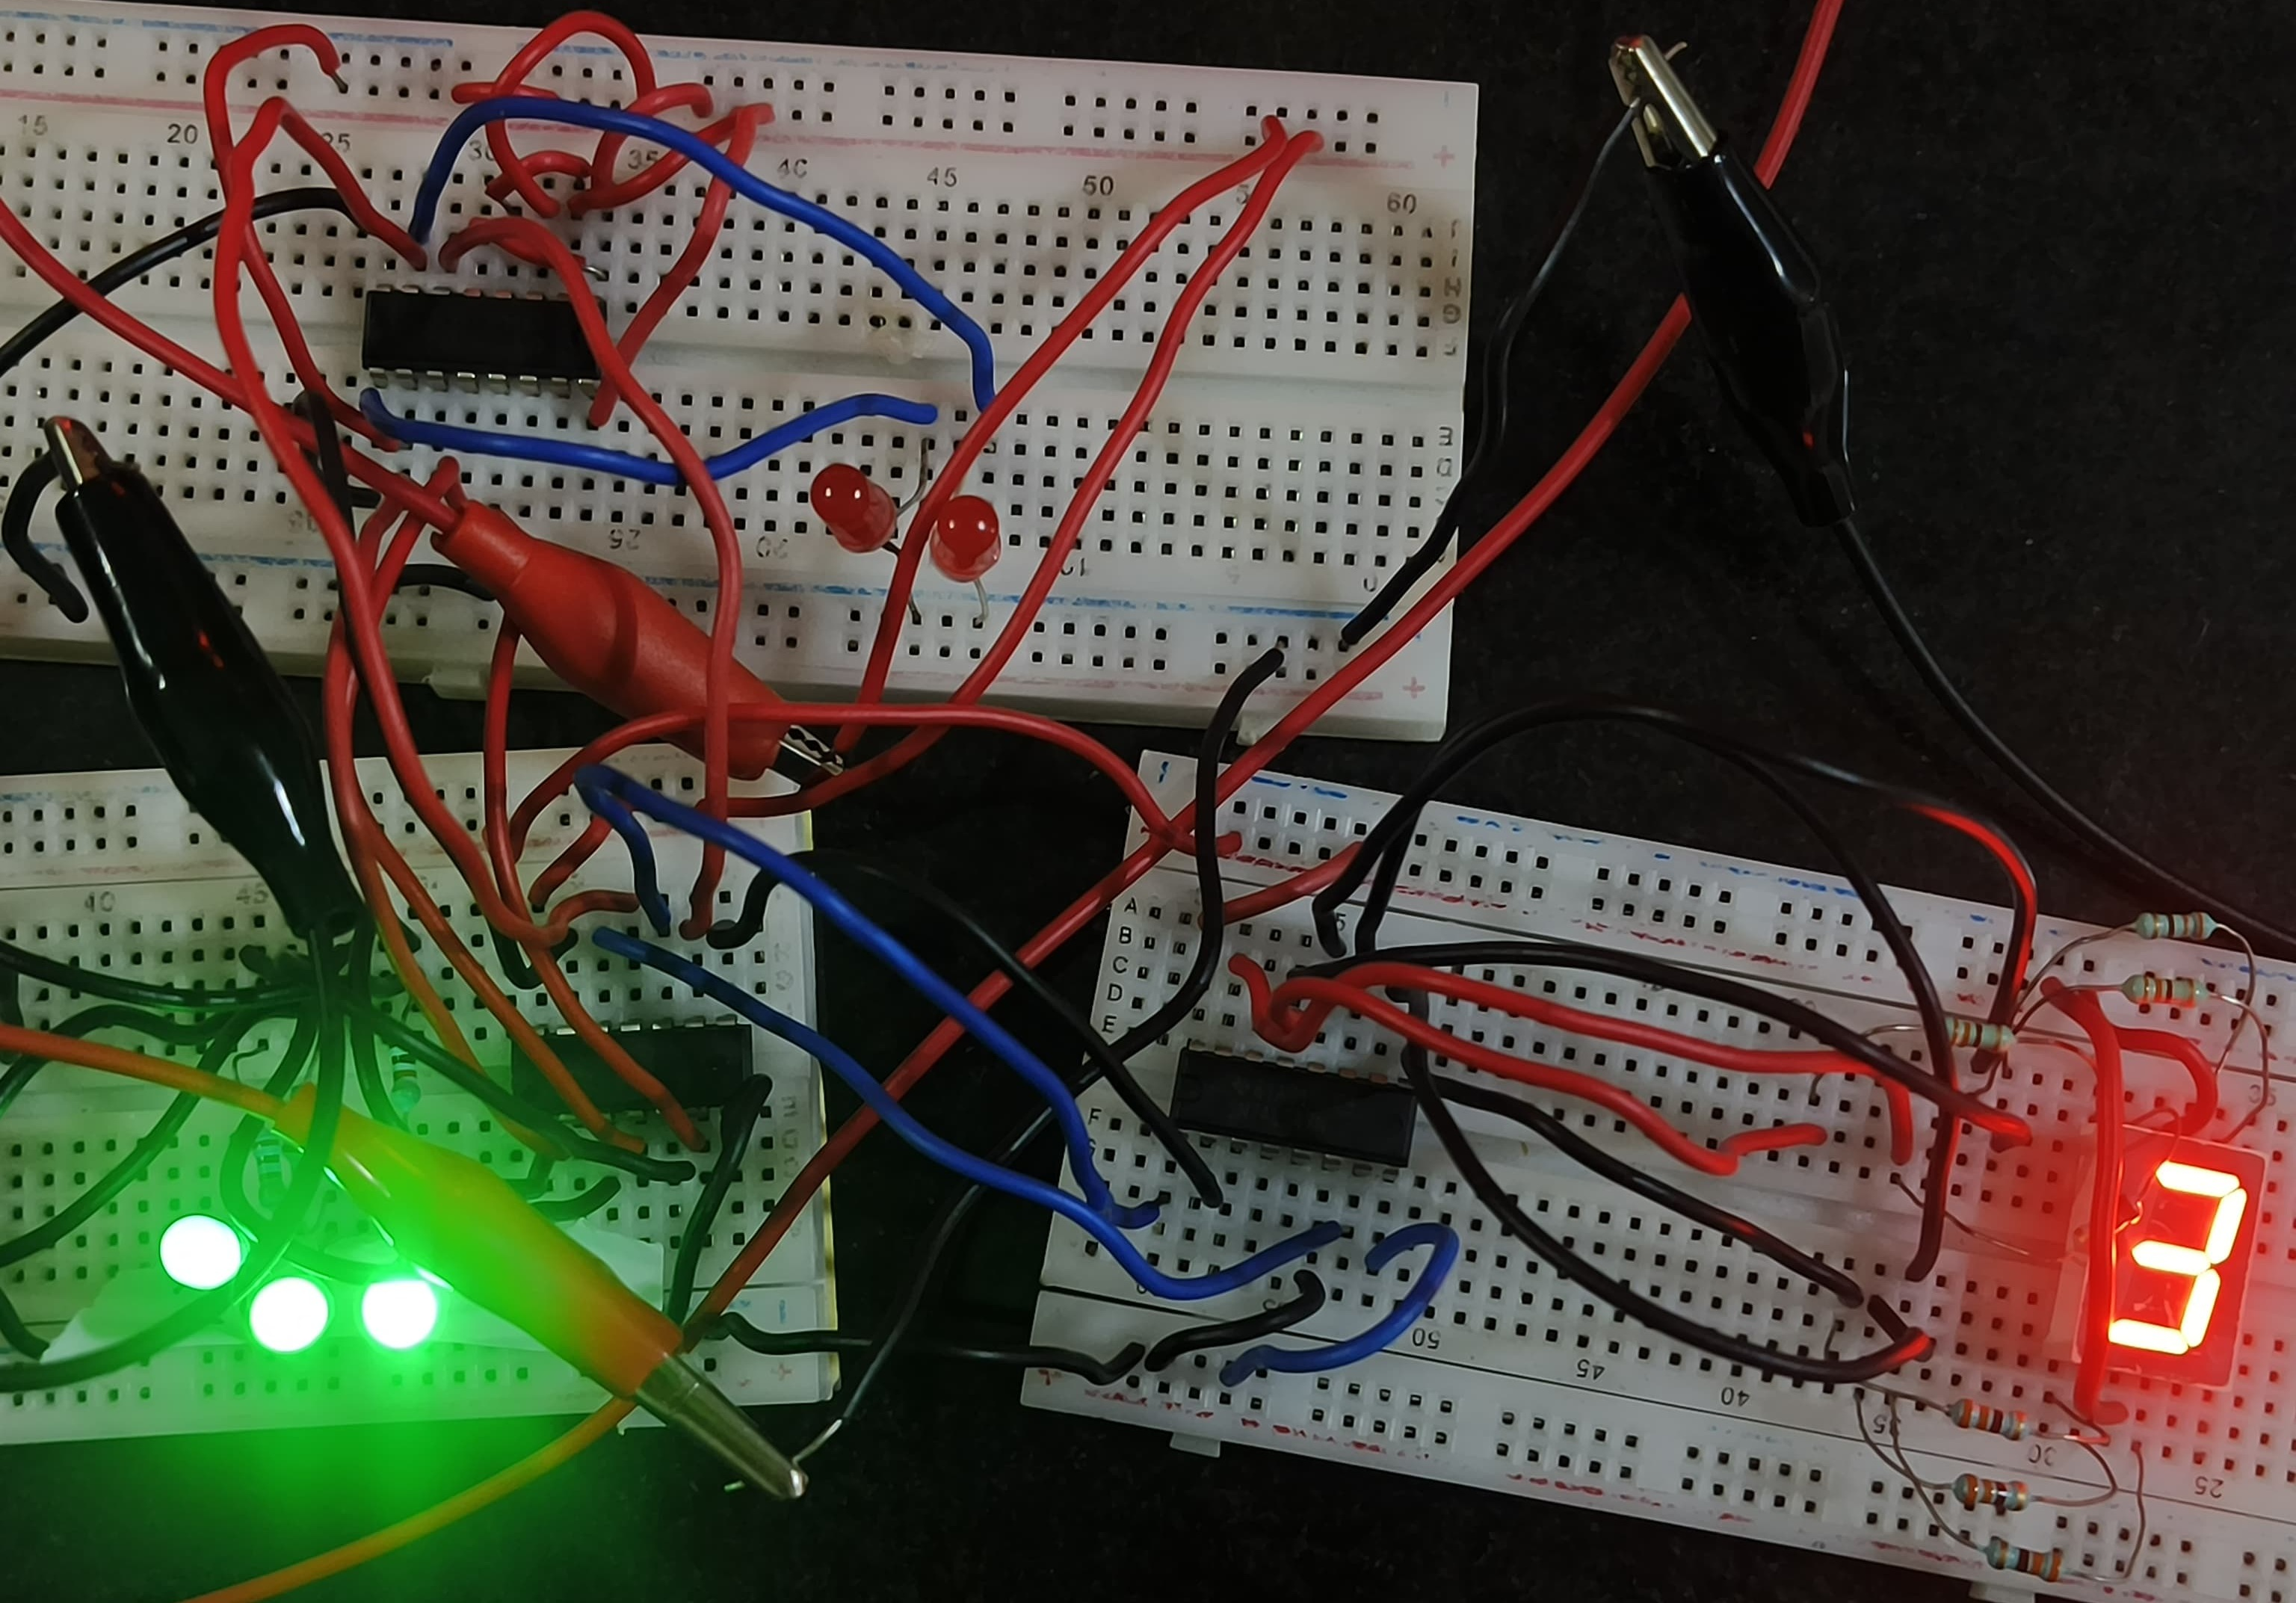
\includegraphics[width=\textwidth]{images/3.JPG}
    \end{subfigure}
    \hfill
    \caption{Three types of earthing points near the SPS building, NISER}
    \label{earth}
\end{figure}